\documentclass[a4paper]{article}

\usepackage{fullpage} % Package to use full page
\usepackage{parskip} % Package to tweak paragraph skipping
\usepackage{tikz} % Package for drawing
\usepackage{amsmath}
\usepackage{hyperref}
\usepackage{listings} % iPackage for code
\usepackage{amsthm}
\usepackage{amsmath}
\usepackage{amssymb}
\usepackage{bbm}

\title{CSC411 Fall 2017\\Assignment 2 Report}
\author{Tianbao Li}
\date{2017/11/04}

\begin{document}

\maketitle

\section{Q1: Class-conditional gaussians}

Given:

\begin{equation}
    p(y=k)=a_k
\end{equation}

\begin{equation}
    p(\mathbf{x}|y=k,\mu,\sigma)=(\prod^d_{i=1}2\pi\sigma^2_i)^{-1/2}\exp\{-\sum^d_{i=1}\frac{1}{2\sigma^2_i}(x_i-\mu_{ki})^2\}
\end{equation}

\subsection{Bayes' rule derivation}

\begin{align*}
    p(y=k|\mathbf{x},\mu,\sigma)&=\frac{p(\mathbf{x}|y=k,\mu,\sigma)p(y=k)}{p(\mathbf{x}|\mu,\sigma)}\\
    &=\frac{p(\mathbf{x}|y=k,\mu,\sigma)p(y=k)}{\sum^K_{j=1}p(\mathbf{x}|y=j,\mu,\sigma)}\\
    &=\frac{(\prod^d_{i=1}2\pi\sigma^2_i)^{-1/2}\exp\{-\sum^d_{i=1}\frac{1}{2\sigma^2_i}(x_i-\mu_{ki})^2\}a_k}{\sum^K_{j=1}(\prod^d_{i=1}2\pi\sigma^2_i)^{-1/2}\exp\{-\sum^d_{i=1}\frac{1}{2\sigma^2_i}(x_i-\mu_{ji})^2\}}
\end{align*}

\subsection{Negative likelihood function (NLL)}

\begin{align*}
    \ell(\theta;D)&=-\log p(y^{(1)},\mathbf{x}^{(1)},y^{(2)},\mathbf{x}^{(2)},\dots,y^{(N)},\mathbf{x}^{(N)}|\theta)\\
    &=-\log\prod^N_{n=1}p(y^{(n)},x^{(n)}|\theta)\\
    &=-\sum^N_{n=1}(\log p(x^{(n)}|y^{(n)},
    \theta)+\log p(y^{(n)}|\theta))\\
    &=-\sum^N_{n=1}(\log((\prod^d_{i=1}2\pi\sigma^2_i)^{-1/2}\exp\{-\sum^d_{i=1}\frac{1}{2\sigma^2_i}(x_i^{(n)}-\mu_{ki})^2\})+\log\alpha_k)\\
    &=-\sum^N_{n=1}(-\frac{1}{2}\sum^d_{i=1}2\pi\sigma^2_i-\sum^d_{i=1}\frac{1}{2\sigma^2_i}(x^{(n)}_i-\mu_{ki})^2+\log\alpha_k)\\
    &=\sum^N_{n=1}(\sum^d_{i=1}\pi\sigma^2_i+\sum^d_{i=1}\frac{1}{2\sigma^2_i}(x^{(n)}_i-\mu_{ki})^2-\log\alpha_k)
\end{align*}

\subsection{Partial derivatives}

\begin{align*}
    \frac{\partial \ell}{\partial \mu_{ki}}&=\frac{\partial(\sum^N_{n=1}\sum^d_{i=1}\frac{1}{2\sigma^2_i}(x^{(n)}_i-\mu_{ki})^2)}{\partial \mu_{ki}}\\
    &=-\sum^N_{n=1}\sum^d_{i=1}\frac{1}{\sigma^2_i}\mathbbm{1}(y^{(n)}=k)(x^{(n)}_i-\mu_{ki})\\
    \frac{\partial \ell}{\partial \sigma_i^2}&=\frac{\partial(\sum^N_{n=1}(\sum^d_{i=1}\pi\sigma^2_i+\sum^d_{i=1}\frac{1}{2\sigma^2_i}(x^{(n)}_i-\mu_{ki})^2))}{\partial \sigma_i^2}\\
    &=\sum^N_{n=1}\sum^d_{i=1}\mathbbm{1}(y^{(n)}=k)(2\pi-\frac{1}{2\sigma^4_i}(x^{(n)}_i-\mu_{ki})^2)
\end{align*}

\subsection{Estimation}

\begin{align*}
    \frac{\partial \ell}{\partial \mu_{ki}}&=0\\
    \Rightarrow\mu_{ki}&=\frac{\sum^N_{n=1}\sum^d_{i=1}\mathbbm{1}(y^{(n)}=k)x^{(n)}_i}{\sum^N_{n=1}\sum^d_{i=1}\mathbbm{1}(y^{(n)}=k)}\\
    \frac{\partial \ell}{\partial \sigma_i^2}&=0\\
    \Rightarrow\sigma_i&=\sqrt[4]{\frac{\sum^N_{n=1}\sum^d_{i=1}\mathbbm{1}(y^{(n)}=k)*(x^{(n)}_i-\mu_{ki})^2}{\sum^N_{n=1}\sum^d_{i=1}\mathbbm{1}(y^{(n)}=k)*4\pi}}
\end{align*}

\section{Handwritten digit classification}

In this assignemnt, we use the dataset of handwritten digit. To get a macro view of the data, here we plot the means for each data classes in the training set, shown in Figure~\ref{fig: Trainging_data_mean}.

\begin{figure}[htbp]
\centering
\includegraphics[width = 8cm]{Trainging_data_mean}
\caption{Mean for each class}
\label{fig: Trainging_data_mean}
\end{figure}

\subsection{K-NN classifier}

Fisrt, we build a K nearest neighbor classifier using Euclidean distance on the data.

\subsubsection{Accuracy for certain K values}

\begin{itemize}
    \item for K = 1
    \begin{itemize}
        \item train classification accuracy: 1.0
        \item test classification accuracy: 0.96875
    \end{itemize}
    \item for K = 15
    \begin{itemize}
        \item train classification accuracy: 0.961
        \item test classification accuracy: 0.959
    \end{itemize}
\end{itemize}

\subsubsection{Ties solution}

During the implementation, one important problem is that ties usually happens and need to be broken. The solution is shown as follows.

\begin{lstlisting}[language = Python]
    def query_knn(self, test_point, k):
        digit = None
        dist = self.l2_distance(test_point)
        noTies = False
        while noTies == False:
            mink = np.argpartition(dist, k)[:k]
            counts = np.bincount(self.train_labels[mink].astype(int))
            digit = np.argwhere(counts == np.amax(counts))
            if len(digit) > 1:
                k = k - 1
            else:
                noTies = True
        return digit
\end{lstlisting}

While running KNN, if ties happen (which means two classes has the same maximum count), we try to decrease k by 1 and run the KNN again until no ties. As the class label should focus on one or a few classes, ties are unlikely to happen when $K=1$, so this should be a solution to get an answer without ties.

\subsubsection{Best k}

Here we implement 10 fold cross validation in range 1-15 to find the optimal K. By finding minimun validation error, optimal K for this problem is that $K=3$ and accuracies are shown as follows.

\begin{itemize}
    \item train classification accuracy: 1.0
    \item valiadation classification accuracy: 0.96514286
    \item test classification accuracy: 0.96875
\end{itemize}


\bibliographystyle{plain}
\bibliography{bibliography.bib}
\end{document}





\subsection{Data loading}

Here, we use function in sklearn.dataset() to read Boston Housing data.

\begin{lstlisting}[language = Python]
def load_data():
    boston = datasets.load_boston()
    X = boston.data
    y = boston.target
    features = boston.feature_names
    return X,y,features
\end{lstlisting}

In the return variables, $X$ is several lines of data on each feature, $y$ is the target value for each line of data, $features$ contains the names of all the features.

\subsection{Data summarization}

The input dataset has the folowing properties:

\begin{itemize}
	\item number of data points: 506
	\item dimensions: 13
	\item features: ['CRIM' 'ZN' 'INDUS' 'CHAS' 'NOX' 'RM' 'AGE' 'DIS' 'RAD' 'TAX' 'PTRATIO' 'B' 'LSTAT']
    \item Mean house price: 22.5328063241
    \item Standard deviation of house price: 9.18801154528
\end{itemize}

\subsection{Feature visualization}

Data distribution on each feature is shown in Figure~\ref{fig: Data distribution}.

\begin{figure}[htbp]
\centering
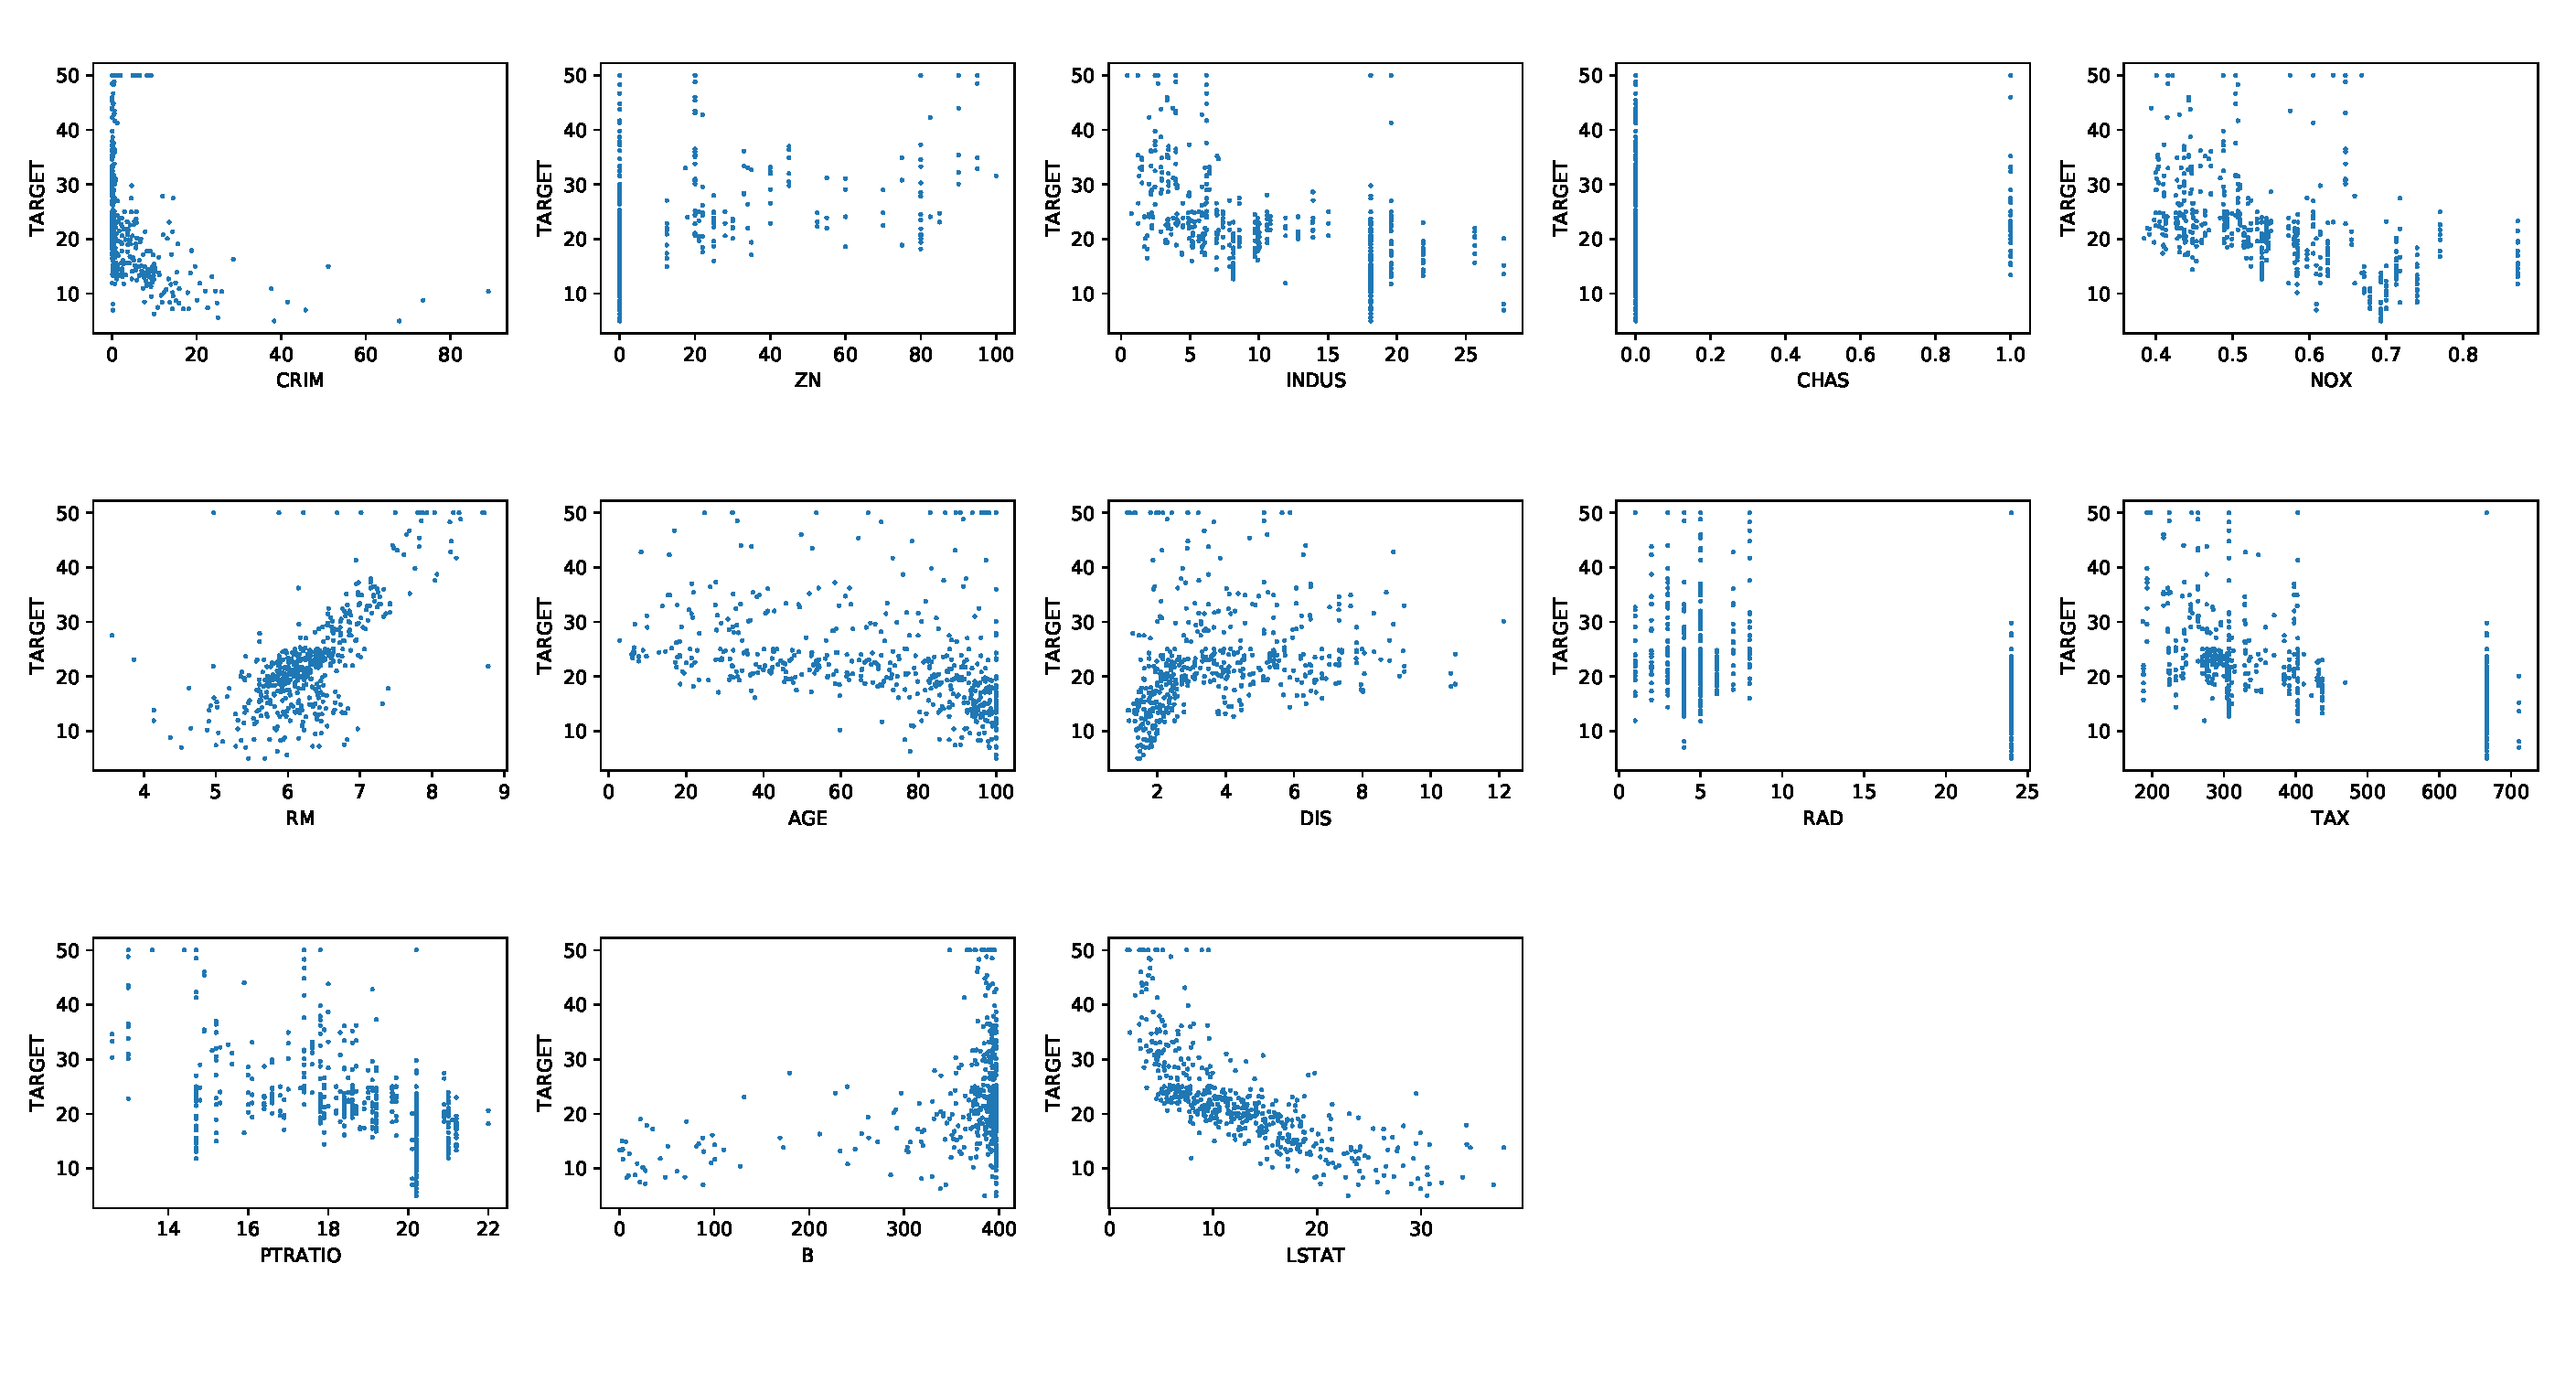
\includegraphics[width = 15cm]{DataDistribution}
\caption{Data points against target for each feature}
\label{fig: Data distribution}
\end{figure}

\subsection{Data division}

To divide training data set and test data set, in Q1, we use function numpy.random.choice() to implement function split\_data(X, y, training\_ratio = 0.2).

\begin{lstlisting}[language = Python]
def split_data(X, y, training_ratio = 0.2):
    test_chosen = np.random.choice(len(X), int(len(X) * training_ratio))
    ......
    return training_set_x, test_set_x, training_set_y, test_set_y
\end{lstlisting}

In the function, we split $X$ and $y$ into $training_set_x$, $test_set_x$, $training_set_y$, $test_set_y$ according to $training_ratio$ for future usage.

\subsection{Linear regression}

To solve linear regression problem and get the weightes $w$, we use numpy.linalg.solve() on the formula:

\begin{equation}
    X^\mathrm{T}Xw^*=X^\mathrm{T}y
\end{equation}

\subsection{Feature weights}

After the calculation, we can get the weight on each feature as shown in Table~\ref{tab: Feature weights}.

\begin{table}[htbp]
\centering
\begin{tabular}{|c|c|c|}
    \hline
    Feature & Weight & Mean\\
    \hline
    CRIM & 41.795688882257188 & 3.5937607114624512\\
    \hline
    ZN & -0.13159561392787489 & 11.363636363636363\\
    \hline
    INDUS & 0.056336470652065491 & 11.136778656126481\\
    \hline
    CHAS & 0.033639549287715828 & 0.069169960474308304\\
    \hline
    NOX & 3.7698365450326135 & 0.55469505928853757\\
    \hline
    RM & -19.35371695539391 & 6.2846343873517787\\
    \hline
    AGE & 3.1091523339672826 & 68.574901185770756\\
    \hline
    DIS & 0.010472276182880488 & 3.7950426877470358\\
    \hline
    RAD & -1.5681353658907364
     & 9.5494071146245059\\
    \hline
    TAX & 0.33065329716511299 & 408.23715415019763\\
    \hline
    PTRATIO & -0.011395113448445227 & 18.455533596837945\\
    \hline
    B & -0.97967928714208496 & 356.67403162055342\\
    \hline
    LSTAT & 0.0096343495439206173 & 12.653063241106722\\
    \hline
    \end{tabular}
\caption{Feature weights}
\label{tab: Feature weights}
\end{table}

Here, we take the feature 'INDUS' (proportion of non-retail business acres per town) as an analysis example. Shown in Table\ref{tab: Feature weights}, we can see feature 'INDUS' has a weight of 0.056336470652065491. As a positive weight, the sign means that is has a positive influence in the target, the housing price. In general ideas, people likes to live in the areas with more shops, which means that house price could be higher. That just fits the result.

\subsection{Model test}
We use $20\%$ of the data as test date to just the fitness of the model. Here are some results of different metics:

\begin{itemize}
    \item MSE: 18.268879264780917
    \item MAE: 3.1172529292203892
    \item R2: 0.75025578036036022
\end{itemize}

These numbers could change due to different training-test dataset division.

\subsection{Feature selection}

To choose the most significan feature, weight of teh featuers are a good metrics. However, due to the different magnitudes of weights, we decide to multiply weight and mean for each feature and use it as the influnce on the target. It is shown as Table~\ref{tab: Feature influence}.

\begin{table}[htbp]
\centering
\begin{tabular}{|c|c|}
    \hline
    Feature & Inluence\\
    \hline
    CRIM & 150.2037046136\\
    \hline
    ZN & -1.4954047037\\
    \hline
    INDUS & 0.6274068039\\
    \hline
    CHAS & 0.0023268463\\
    \hline
    NOX & 2.0911097059\\
    \hline
    RM & -121.6310351009\\
    \hline
    AGE & 213.2098140733\\
    \hline
    DIS & 0.0397427352\\
    \hline
    RAD & -14.9747630197\\
    \hline
    TAX & 134.9849610451\\
    \hline
    PTRATIO & -0.2103028991\\
    \hline
    B & -349.4261610401\\
    \hline
    LSTAT & 0.1219040341\\
    \hline
    \end{tabular}
\caption{Feature weights}
\label{tab: Feature influence}
\end{table}

From the table, we can see that the feature 'B' has the largest absolute value, which means 'B' predicts the price best.

\section{Q2: Locally reweighted regression}

\subsection{$w^*$ solution proof}

Given $(x^{(1)}, y^{(1)}), \dots, (x^{(N)}, y^{(N)})$ and positive weights $a^{(1)}, \dots, a^{(N)}$, show that the solution to the weighted least square ploblem

\begin{equation}
    w^*=\operatorname{argmin}\frac{1}{2}\sum_{i=1}^Na^{(i)}(y^{(i)}-w^\mathrm{T}x^{(i)})^2+\frac{\lambda}{2}\|w\|^2
\end{equation}

is given bu the formula

\begin{equation}
    w^*=(X^\mathrm{T}AX+\lambda I)^{-1}X^\mathrm{T}Ay
\end{equation}

where $X$ is the design matrix (defined in class) and $A$ is a diagonal matrix where $A_{ii}=a^{(i)}$

\begin{proof}
    \begin{align*}
        w^*&=\operatorname{argmin}\frac{1}{2}\sum_{i=1}^Na^{(i)}(y^{(i)}-w^\mathrm{T}x^{(i)})^2+\frac{\lambda}{2}\|w\|^2\\
        L(w^*)&=\frac{1}{2}\sum_{i=1}^Na^{(i)}(y^{(i)}-w^\mathrm{T}x^{(i)})^2+\frac{\lambda}{2}\|w\|^2\\
        &=\frac{1}{2}A\|y-Xw\|^2+\frac{\lambda}{2}\|w\|^2\\
        &=\frac{1}{2}(y-Xw)^\mathrm{T}A(y-Xw)+\frac{\lambda}{2}\|w\|^2\\
        &=\frac{1}{2}(y^\mathrm{T}Ay-2w^\mathrm{T}X^\mathrm{T}Ay+w^\mathrm{T}X^\mathrm{T}AXw)+\frac{\lambda}{2}\|w\|^2\\
        \nabla L(w^*)&=\frac{1}{2}(-2X^\mathrm{T}Ay+2X^\mathrm{T}AXw)+\lambda w\\
        &=X^\mathrm{T}AXw+\lambda w-X^\mathrm{T}Ay\\
    \end{align*}
    \qquad Setting this gradient to zero gives
    \begin{align*}
        X^\mathrm{T}Ay&=X^\mathrm{T}AXw+\lambda w\\
        w^*&=(X^\mathrm{T}AX+\lambda I)^{-1}X^\mathrm{T}Ay
    \end{align*}
\end{proof}

\subsection{LRLS implementation}

Some essential things in LRLS implemented:

\begin{itemize}
    \item $\|x-x^{(i)}\|^2$ in $a^{(i)}$ calculation: using provided function l2(A,B)
    \item solving $w^*$: using numpy.linalg.solve()
    \item avoiding overflows/underflows: adding $-max_jA_j$in square distance calculation
\end{itemize}

\subsection{K-fold corss-validation}

In this question, we choose $\tau$ from$[10, 1000]$ and proceed cross-validation on different $\tau$value. The variation of loss value is shown in Figure~\ref{fig: Tau_loss}. For $\tau$ in$[10, 1000]$, mean value of the loss is 16.9512301253, and the minimun value of the loss is 11.9637899295.

\begin{figure}[htbp]
\centering
\includegraphics[width = 8cm]{tau-lossvalue}
\caption{Loss value for each $\tau$}
\label{fig: Tau_loss}
\end{figure}

From the figure we can see that, loss value has the following tending:

\begin{itemize}

    \item when $\tau \to 0$, loss value tends towards $+\infty$
    \item when $\tau \to +\infty$, loss value tends towards a certain small value
\end{itemize}

\begin{proof}
    \begin{align*}
        a^{(i)}&=\frac{e^{-\frac{\|x-x^{(i)}\|^2}{2\tau^2}}}{\sum_je^{-\frac{\|x-x^{(j)}\|^2}{2\tau^2}}}\\
        \frac{1}{a^{(i)}}&=\frac{\sum_je^{-\frac{\|x-x^{(j)}\|^2}{2\tau^2}}}{e^{-\frac{\|x-x^{(i)}\|^2}{2\tau^2}}}\\
        &=1+\frac{\sum_{i\neq j}e^{-\frac{\|x-x^{(j)}\|^2}{2\tau^2}}}{e^{-\frac{\|x-x^{(i)}\|^2}{2\tau^2}}}\\
        &=1+\sum_{i\neq j}\frac{e^{-\frac{\|x-x^{(j)}\|^2}{2\tau^2}}}{e^{-\frac{\|x-x^{(i)}\|^2}{2\tau^2}}}\\
        &=1+\sum_{i\neq j}e^{\frac{\|x-x^{(i)}\|^2-\|x-x^{(j)}\|^2}{2\tau^2}}\\
    \end{align*}
    \begin{align*}
        when\quad\tau&\to 0,\frac{1}{a^{(i)}}\to+\infty, a^{(i)}\to 0,A\to 0\\
        when\quad\tau&\to +\infty,\frac{1}{a^{(i)}}\to1+\sum_{i\neq j}1=N, a^{(i)}\to\frac{1}{N},A\to \frac{1}{N}I\\
    \end{align*}
    \begin{align*}
        \because w^*&=\frac{X^\mathrm{T}Ay}{X^\mathrm{T}AX+\lambda I}\\
        \therefore loss&=(\hat{y}-y)^2\\
        &=(X^\mathrm{T}w^*-y)^2\\
        &=(\frac{X^\mathrm{T}AXy}{X^\mathrm{T}AX+\lambda I}-y)^2\\
        &=(\frac{\lambda Iy}{X^\mathrm{T}AX+\lambda I})^2\\
    \end{align*}
    \begin{align*}
        when\quad\tau&\to 0,A\to 0,loss\to 0\\
        when\quad\tau&\to +\infty,A\to \frac{1}{N}I,loss\to (\frac{\lambda Iy}{\frac{1}{N}X^\mathrm{T}IX+\lambda I})^2=(\frac{N\lambda y}{X^\mathrm{T}X+\lambda })^2\\
    \end{align*}
\end{proof}

\section{Q3: Mini-batch SGD gradient estimator}

\subsection{Mini-batch mean value proof}

Given a set $\{a_1, \dots, a_n\}$ and random mini-batchs $\mathcal{I}$ of size $m$, show that

\begin{equation}
    \mathbb{E}_{\mathcal{I}}[\frac{1}{m}\sum_{i\in \mathcal{I}}a_i]=\frac{1}{n}\sum_{i=1}^na_i
\end{equation}

\begin{proof}
    \qquad As $a_i$ is randomly sampled
    \begin{align*}
        p(a_1)&=p(a_2)=\dots=p(a_i)=\dots=p(a_n)\\
        \mathbb{E}(a_1)&=\mathbb{E}(a_2)=\dots=\mathbb{E}(a_i)=\dots=\mathbb{E}(a_n)
    \end{align*}

    \begin{align*}
        \therefore\mathbb{E}_{\mathcal{I}}[\frac{1}{m}\sum_{i\in \mathcal{I}}a_i]&=\frac{1}{m}\mathbb{E}_{\mathcal{I}}[\sum_{i\in \mathcal{I}}a_i]\\
        &=\frac{1}{m}[\mathbb{E}(a_1)+\dots+\mathbb{E}(a_m)]\\
        &=\frac{1}{m}*[m*\mathbb{E}(a)]\\
        &=\mathbb{E}(a)\\
        &=\frac{1}{n}\sum_{i=1}^na_i
    \end{align*}
\end{proof}

\subsection{Mini-batch gradient proof}

Show that $\mathbb{E}_\mathcal{I}[\nabla L_{\mathcal{I}}(x,y,\theta)]=\nabla L(x,y,\theta)$

\begin{proof}
    \begin{align*}
        \mathbb{E}_\mathcal{I}[\nabla L_{\mathcal{I}}(x,y,\theta)]&=\mathbb{E}_\mathcal{I}[\nabla(\frac{1}{m}\sum_{i\in\mathcal{I}}\ell(x^{(i)},y^{(i)},\theta))]\\
        &=\frac{1}{m}\mathbb{E}_\mathcal{I}[\nabla(\sum_{i\in\mathcal{I}}\ell(x^{(i)},y^{(i)},\theta))]\\
        &=\frac{1}{m}\mathbb{E}_\mathcal{I}[\sum_{i\in\mathcal{I}}\nabla\ell(x^{(i)},y^{(i)},\theta)]\\
        &=\frac{1}{m}\mathbb{E}_\mathcal{I}[\sum_{i\in\mathcal{I}}\ell(x^{(i)},y^{(i)},\theta+\Delta\theta)-\ell(x^{(i)},y^{(i)},\theta)]\\
        &=\frac{1}{m}\mathbb{E}_\mathcal{I}[(\ell(x^{(1)},y^{(1)},\theta+\Delta\theta)-\ell(x^{(1)},y^{(1)},\theta))+\dots\\&\qquad+(\ell(x^{(m)},y^{(m)},\theta+\Delta\theta)-\ell(x^{(m)},y^{(m)},\theta))]\\
        &=\frac{1}{m}[\mathbb{E}(\ell(x^{(1)},y^{(1)},\theta+\Delta\theta)-\ell(x^{(1)},y^{(1)},\theta))+\dots\\&\qquad+\mathbb{E}(\ell(x^{(m)},y^{(m)},\theta+\Delta\theta)-\ell(x^{(m)},y^{(m)},\theta))]\\
        &=\frac{1}{m}[m*\mathbb{E}(\ell(x,y,\theta+\Delta\theta)-\ell(x,y,\theta))]\\
        &=\mathbb{E}(\ell(x,y,\theta+\Delta\theta)-\ell(x,y,\theta))\\
        &=\mathbb{E}(\nabla\ell(x,y,\theta))\\
        \nabla L(x,y,\theta)&=\nabla[\frac{1}{n}\sum_{i=1}^n\ell(x^{(i)},y^{(i)},\theta)]\\
        &=\frac{1}{n}\sum_{i=1}^n\nabla\ell(x^{(i)},y^{(i)},\theta)\\
        &=\mathbb{E}(\nabla\ell(x,y,\theta))
    \end{align*}
    \begin{equation*}
        \therefore\mathbb{E}_\mathcal{I}[\nabla L_{\mathcal{I}}(x,y,\theta)]=\nabla L(x,y,\theta)
    \end{equation*}
\end{proof}

\subsection{Mini-batch expectations}

As the proofs above, expectations of mean value and gradient of mini-batch is just the same like the ones of full-batch, which means different data choices of mini-batch and full-batch return the same result.

\subsection{Gradient implementation}

For loss funtion $\ell(x,y,w)=(y-w^{\mathrm{T}}x)^2$, its gradient can be presented as:

\begin{equation}
    \nabla\ell(x,y,w)=2x(w^{\mathrm{T}}x-y)
\end{equation}

In the code implementation, gradient is computed by the formula above.

\subsection{Mini-batch gradient VS true gradient}

In this part, we set $m=50$ and $K=500$. To compare the gradient value between mini-batch and the true gradient (entire data set), we use following metrics:

\begin{itemize}
    \item squared distance metric: 36232.487235814442
    \item cosine similarity: 0.99999783659754915
\end{itemize}

For these two metrics, cosine similarity is a more meaningful measure in this case. Square distance metric is hard to judge just because we can not tell the difference simply from one value. However, for cosine similarity valued in $[0,1]$, value tending to 1 means the gradients are very similar. We can easily judge this.

\subsection{Affect of batch size}

Here, we give out the figures of $\log\tilde{\sigma}_j$ against $\log(m)$ on all features to show the influence of batch size om the gradient varience. It is shown as Figure~\ref{fig: M VS gradient variance}.

\begin{figure}[htbp]
\centering
\includegraphics[width = 15cm]{m-gradvar}
\caption{Log(m) against log(gradient variance) for each feature}
\label{fig: M VS gradient variance}
\end{figure}
